% ===== 原文 pp.90--93（tr-07a）=====
% 起点说明：p.89 末句 "…and one" 于 p.90 首句续完（Lead 裁决：由 tr-07 收尾），
% 故本片段第一句为跨页句的续文，其后自 p.90 第二段起照常续写。

% [原文 p.90]
就得到 $\gamma$ 上的 Verlinde 圈，它由插入与该缺陷相关联的顶点算子 $V_\alpha$ 并使其绕 $\gamma$ 移动而构造出来。

% [Tutor Note: p.90 的 $\alpha$ 是余维 2 缺陷（orbifold 型面算子）在 $\mathfrak{t}$ 中的参数；
% 其连续部分即畴壁上未破缺规范群 $H$ 的 FI 参数，离散部分对应"非满"缺陷的额外装饰。
% 核对方式：顶点算子沿 $\gamma$ 移动给出 Verlinde 圈，其表示由 $\alpha$ 的离散部分（权）确定；
% $\alpha$ 连续变化时圈算子应连续变形，这与 8.2 小节 Wilson/'t Hooft 圈的参数化一致。]
$\alpha$（它属于余维 2 缺陷）的连续参数是畴壁上未破缺规范对称性 $H$ 的 FI 参数。一般的顶点算子还可以包含离散部分；相应地，非满的驯服余维 2 缺陷可以用生活在其余维 4 世界体积上的额外余维 4 缺陷来装饰。在当前的构造中，这导致 $H$ 的两个表示 $R_1$ 与 $R_2$ 中的 Wilson 圈算子，它们分别位于 8.2 小节的两条圆周上。除非 $R_1$（相应地 $R_2$）本身就是 $G$ 的表示，这些圈会被粘在畴壁上。

\para{Janus 畴壁。}
我们的第二个构造不涉及余维 2 或余维 4 算子。取而代之，我们把 $\cX(\fg)$ 放在 $S^4_b\times C$ 上，其中 $C$ 的复结构随 $S^4_b$ 的纬度变化 [43]。这保留了超对称的一半；而在变化急剧地发生在赤道（或某条纬线）上的极限下，我们在 4d 理论中得到所谓的 Janus 畴壁 [602--607]。这是具有不同规范耦合的 class S 理论之间的半 BPS 界面。带此界面的配分函数具有通常的因子化形式 (1.7)：全纯与反全纯贡献分别来自极点，但每个因子中使用的规范耦合并非彼此的复共轭。相应地，CFT 关联函数 (1.9) 变为对全纯因子与反全纯因子使用不同的复结构。

\para{S 对偶畴壁。}
通过调节规范耦合，我们可以得到彼此 S 对偶的理论。若在两侧切换到同一个 S 对偶标架，我们就得到一个称为 S 对偶畴壁 [608] 的 3d 算子，它两侧是同一个理论（且规范耦合相同）。在 4d 理论中插入一个 S 对偶畴壁，在 2d 这边相当于对全纯（或反全纯）共形块做一个模变换（融合、编织、S-移动）。这与我们在 9.3 小节讨论的 3d/3d 对应的某些特例 [87, 89, 609, 610] 有关。S 对偶畴壁与圈算子之间有相互作用：在适当的意义下，它把畴壁一侧的 Wilson 圈变换为另一侧的 't Hooft 圈。

例如，4d $\cN=4$ SYM 的 S 对偶畴壁等价于把 3d $\cN=4$ 理论 $T[G]$ 与畴壁两侧的 SYM 耦合起来 [608]，而 S-移动核被预期 [86] 与 $T[G]$ 的 $S^3_b$ 配分函数相符。对 $\fg=\fsu(N)$，该畴壁理论是一个 3d $\cN=4$ 线性箭图，
% [Tutor Note: (8.11) 方括号里是箭图：节点 N, N−1, …, 1 依次相连，N 为方框、其余为圆/椭圆节点
% （原文由 LaTeX 宏绘制；这里用 TikZ 重画，节点标签与连线照抄原图）。
% 等式右边说明该 $S^3_b$ 配分函数等于 $W_N$ 代数的 S-移动（braiding）核。
% 核对锚点：$N=2$ 时 $W_2=$ Virasoro，其 S-移动核应与 [611, 612] 的四点 Virasoro 编织核相符------
% 这也正是下文 SU(2) SQCD（$N_f=4$）情形的依据。]
\begin{equation}
Z_{S^3_b}\left[\;
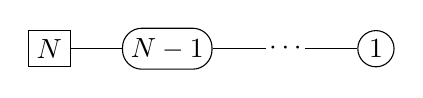
\begin{tikzpicture}[baseline=(current bounding box.center)]
  \node[draw,rectangle,inner sep=3pt] (a) at (0,0) {$N$};
  \node[draw,rounded corners=7pt,inner sep=3pt,minimum width=1.05cm,minimum height=0.52cm] (b) at (1.5,0) {$N-1$};
  \node (c) at (3.0,0) {$\cdots$};
  \node[draw,circle,inner sep=1pt,minimum size=0.46cm] (d) at (4.15,0) {$1$};
  \draw (a.east)--(b.west);
  \draw (b.east)--(2.75,0);
  \draw (3.25,0)--(d.west);
\end{tikzpicture}
\;\right]=(W_N\ \text{algebra S-move kernel}).
\tag{8.11}
\end{equation}

Virasoro 四点共形块已知的编织核 [611, 612] 导出了对 4d $\cN=2$ SU(2) SQCD（$N_f=4$）的 S 对偶畴壁的一种描述 [88]：它是一个 3d $\cN=2$ SU(2) SQCD（$N_f=6$），与两侧的 4d 理论作适当耦合。

对 $W_N$ 四点共形块的编织核作自举（bootstrap），导出了对 SU($N$) SQCD 的 S 对偶畴壁的一种描述 [90]：它是 U($N-1$) SQCD（其中带有 [613] 中已理解的 3d 单极子超势），通过三次超势与畴壁两侧的 4d 理论耦合起来，
% [原文 p.91]
% [Tutor Note: (8.12) 是三维箭图：中间一行是 U(N−1) ← 2N；U(N−1) 竖直向上、向下各接一个圆节点 N，
% 两个 N 还分别与右侧 2N 方框以斜线相连；上下两个 N 旁标 "4d"，表示它们与两侧 4d 理论耦合。
% 按原图用 TikZ 重画。物理核对：去掉 4d 节点后剩下 3d N=2 的 U(N−1) 规范理论配 2N 个基本超多重态，
% 正是 SU(N) SQCD 的 S 对偶壁（对偶群 U(N−1)、味数 2N），与正文 "U(N−1) SQCD" 的说法一致。]
\begin{equation}
Z\;
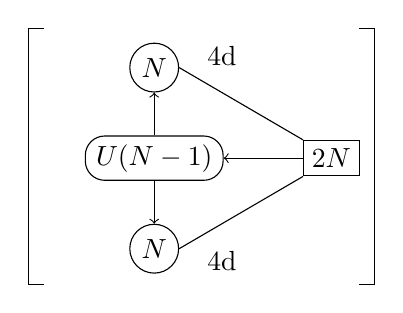
\begin{tikzpicture}[baseline=(current bounding box.center)]
  \node[draw,rounded corners=7pt,inner sep=3pt,minimum width=1.75cm,minimum height=0.55cm] (U) at (1.25,0.95) {$U(N-1)$};
  \node[draw,circle,inner sep=1pt,minimum size=0.62cm] (Nt) at (1.25,2.1) {$N$};
  \node[draw,circle,inner sep=1pt,minimum size=0.62cm] (Nb) at (1.25,-0.2) {$N$};
  \node[draw,rectangle,inner sep=3pt] (V) at (3.5,0.95) {$2N$};
  \draw[->] (U.north) -- (Nt.south);
  \draw[->] (U.south) -- (Nb.north);
  \draw[->] (V.west) -- (U.east);
  \draw (V.north west) -- (Nt.east);
  \draw (V.south west) -- (Nb.east);
  \node[anchor=west] at (1.8,2.25) {4d};
  \node[anchor=west] at (1.8,-0.35) {4d};
  \draw (-0.15,2.6) -- (-0.35,2.6) -- (-0.35,-0.65) -- (-0.15,-0.65);
  \draw (3.85,2.6) -- (4.05,2.6) -- (4.05,-0.65) -- (3.85,-0.65);
\end{tikzpicture}
\;=(W_N\ \text{algebra braiding kernel}).
\tag{8.12}
\end{equation}

与 $T[G]$ 理论一样，这个 3d $\cN=2$ 理论（孤立地看，即在解耦 4d 场之后）允许众多对偶 [614]。5d 理论的对偶壁此前已在 [615, 616] 中研究过。

\para{边界 CFT。}
我们前面提到过轨形。除了对 4d 空间作轨形，还可以对一个 $\Z_2$ 对称性作轨形，该对称性表现为关于 $S^4_b$ 赤道的反射以及对黎曼面的反射（以便保持 $\cX(\fg)$ 的手征性）。这导致带边黎曼面与不可定向黎曼面上的 AGT 对应 [91, 92]。在规范理论一侧，人们同时得到定义在压扁半球 $HS^4_b$ 上的若干规范场和定义在压扁射影空间 $\R P^4_b$ 上的另一些规范场。半球配分函数已在 [617] 中算出，而射影空间配分函数则在 [91] 中通过 [249, 250] 进一步探讨的粘合技术得到。

边界算子的纳入尚未被完全阐明。突破迄今处理的 $\fg=\fsu(N)$ 情形也会很有意思，例如理解（5.38）处讨论的双重覆盖（double-cover）构造如何与产生黎曼面边界的 $\Z_2$ 商相互作用。

% [Tutor Note: p.91 §9 引言中 "C a Riemann surface with punctures which extra data D" 一句原文有笔误：
% which 疑应为 with（意为"带穿刺点与额外数据 D"）。这里按 with 的语义翻译而保留原句结构；
% 依据：全书他处（如 p.12、p.97）均写 $\mathrm{T}(\fg,C,D)$，且 $D$ 是附加在穿刺点上的数据，语法上不会用 which 引导。]
\section{其他几何}

\begin{keybox}{在其他一些几何中的 AGT 对应}
\begin{itemize}[leftmargin=1.4em,itemsep=1pt,topsep=1pt]
  \item 对 class S 理论的 5d $\cN=1$ 提升，$Z_{\text{inst}}$ 与 $Z_{S^5}$ 均与 $q$-形变的 Toda 共形块及关联函数相符。提升到 6d 则与 $(q,t)$-形变的 Toda 理论相符。
  \item $\mathrm{T}(\fg,C,D)$ 的 $S^3\times S^1$ 配分函数（超共形指标）与 $C$ 上的一个 TQFT 关联函数相符。
  \item $\cX(\fg)$ 在 $C_3$ 上的扭曲约化给出 3d $\cN=2$ 理论，其 $Z_{S^2\times S^1}$、$Z_{S^3}$ 或透镜空间配分函数与 $\fg_{\C}$ 上的复 Chern--Simons 理论在能级 0、1 或 $k$ 处相符。
  \item M5 膜探测 $\Z_k$ 奇点的 6d $(1,0)$ SCFT 定义了类似于 class S 的 class $S_k$ 4d $\cN=1$ 理论。
\end{itemize}
\end{keybox}

class S 理论 $\mathrm{T}(\fg,C,D)$ 是通过把 $\fg$ 型的 6d $(2,0)$ 理论紧化在 $M_4\times C$ 上得到的，其中 $C$ 是带穿刺点与额外数据 $D$ 的黎曼面。迄今为止我们已广泛讨论了 $M_4=S^4_b$ 的情形及其构造单元 $M_4=\R^4_{\epsilon_1,\epsilon_2}$------对它们而言，配分函数分别等于 2d CFT 的关联函数与共形块。

我们首先讨论这些 4d 可观测量的 5d 提升，即提升到 $\R^4\times S^1$、$S^4\times S^1$ 与 $S^5$ 的（形变）上，这与 $q$-形变有关\footnote{5d 提升中出现的参数 $q$ 与描述 $C$ 之复结构的规范耦合参数无关。事实上我们不再需要为这个规范耦合引入记号。}（9.1 小节）。然后我们改变几何：先把超共形指标------即 $M_4=S^3\times S^1$ 上的配分函数------与（某种推广的）$q$-Yang--Mills TQFT 关联函数联系起来（9.2 小节）；再改为紧化在乘积 $M_3\times C_3$ 与 $M_2\times C_4$ 上，其中"内部"流形 $C$ 是一个双曲三维流形（9.3 小节）或一个四维流形（9.4 小节）。在最后这个小节里，我们还会提及超对称更少的一些推广，以及几个收效较少的几何设置。

% [原文 p.92]
\subsection{升到 5d 与 q-Toda}

这里我们简要综述：把 4d $\cN=2$ 理论提升到 5d $\cN=1$ 如何等价于 2d 理论的 $q$-形变。综述见 [151]。\footnote{感谢 Fabrizio Nieri 详尽地回答了我的问题。}

\para{瞬子配分函数。}
用来定义 Nekrasov 瞬子配分函数 [12, 13] 的 4d $\cN=2$ Omega 背景，可以方便地用 5d $\cN=1$ 的提升来表达：把理论放在 $\R^4\times S^1$ 上，绕 $S^1$ 取扭结边界条件，使得 $\R^4$ 在两个二维平面内分别按 $q$ 与 $t$ 旋转，并额外做一个 R 对称性的扭转以保留部分超对称。更确切地说，$|q|=|t|=1$ 时的这个定义可以通过打开额外的超引力场延拓到复的 $q,t$。5d 提升把 $Z_{\text{inst}}$ 中的所有因子从质量与 Coulomb 分支参数的有理函数变形为三角函数。人们自然会问：AGT 对应的 Toda CFT 一侧该如何形变才能容纳这一点。

人们发现，5d（也称 K-理论）的 $Z_{\text{inst}}$ 是 $q$-形变 W 代数的手征块 [35, 113, 229, 340, 341, 618--620]：Virasoro 代数与 W 代数的相关形变在很久以前就被构造出来了 [621--624]（近代构造见 [625]）。\footnote{与 4d 一样，采用 U($N$) 而非 SU($N$) 规范群会使 $Z_{\text{inst}}$ 更易处理；相应地，人们使用 Ding--Iohara 代数------它是 $\fg$ 型 $qW$ 代数的（泛包络代数的）一个小扩张 [267]。}当质量与 Coulomb 分支参数被适当量子化时，可以用 $qW_N$ 共形块的 Dotsenko--Fateev 积分表示来证明这一等式 [67, 304, 307, 342, 626]（[627] 也用到它）。另见 [272, 628]。
% [Tutor Note: 脚注 69 的 Ding--Iohara 代数即后文 p.101 所论 DIM 代数中的 DI 部分
% （Ding--Iohara--Miki）；这一点在阅读 p.101--102 的代数清单时是重要锚点。]

5d $\cN=1$ 箭图规范理论可以用 IIB 弦论中的 $(p,q)$ 五膜网来实现 [7]。施加 S 对偶会交换 D5 膜与 NS5 膜的角色，从而把 SU($N$)$^{M-1}$ 线性箭图规范理论的 $Z_{\text{inst}}$ 等同于 SU($M$)$^{N-1}$ 的相应量（$M=N=2$ 的证明见 [629]）。这个 5d 谱对偶（也称纤维-底空间对偶，fiber-base duality [630]）一般地把不同 $qW_N$ 理论的手征块联系起来 [631, 632]；它蕴含 3d 镜像对称的某些实例 [585]，以及自旋链之间的关系 [633]。阅读文献时应当留意采用的是两个谱对偶标架中的哪一个，解释见 [634]。

4d 情形作为极限 $q\to 1$ 被取回，其中 $t=q^{-\beta}$，且固定的 $-\beta=b^2=\epsilon_1/\epsilon_2$ 给出 4d 形变参数。除 $q,t\to 1$ 之外还存在其他有趣的极限，尤其是取 $q$ 与 $t$ 为 $k$ 次单位根时，得到 [29, 33, 35--37, 85, 635] 中研究的 $\C^2/\Z_k$ ALE 空间上的 Nekrasov 配分函数。另一个简化极限是 Hall--Littlewood 极限 $q\to 0$ [281, 282]。
% [Tutor Note: 4d 极限的核对锚点：$t=q^{-\beta}$ 且 $-\beta=b^2=\epsilon_1/\epsilon_2$，
% 即 5d 两个参数在 $q\to1$ 时的对数比 $\ln t/\ln q\to-\beta=b^2$。
% 注意此式依赖 5d 的 $q,t$ 约定（哪个平面配 $q$、指数是否带负号）：
% 若取 $q=\ee^{R\epsilon_1},\,t=\ee^{-R\epsilon_2}$，则 $\ln t/\ln q=-\epsilon_2/\epsilon_1=-1/b^2$，
% 与原文的 $-b^2$ 相差倒数与符号。因此回到 4d 时务必先固定 $q,t$ 的定义；
% 本书 p.52 给出的 $\epsilon_1=b/r,\ \epsilon_2=1/(rb)$（故 $b^2=\epsilon_1/\epsilon_2$）才是 4d 参数的权威约定。]

% [原文 p.93]
$Z_{\text{inst}}$ 与 $qW_N$ 共形块的一个与此无关的应用是构造 $q$-Painlevé 方程的解 [636--639]，一如 4d 情形。

\para{紧致配分函数。}
现在让我们把瞬子配分函数粘合起来。$S^4$ 上的配分函数包含来自超荷平方的两个不动点的一对瞬子贡献；与此不同，$S^5$ 上 5d $\cN=1$ 理论的配分函数把三个 K-理论瞬子配分函数组合起来，因为超荷有三个不动圆 [640]。概略地写为
\begin{equation}
Z_{S^5}=\int \dd a\, Z_{\text{pert}}Z_{\text{inst},1}Z_{\text{inst},2}Z_{\text{inst},3}.
\tag{9.1}
\end{equation}
压扁的 $S^5$ 有三个轴长 $\omega_1,\omega_2,\omega_3$，这里不同的 $Z_{\text{inst},i}$ 分别在参数 $(q,t)$ 取
$\big(\tfrac{\omega_2}{\omega_1},\tfrac{\omega_3}{\omega_1}\big)$、$\big(\tfrac{\omega_1}{\omega_2},\tfrac{\omega_3}{\omega_2}\big)$、$\big(\tfrac{\omega_1}{\omega_3},\tfrac{\omega_2}{\omega_3}\big)$ 的 $\Omega$ 背景中计算。
% [Tutor Note: (9.1) 的三个 $\Omega$ 背景参数核对：三组比值满足
% $(\omega_2/\omega_1)(\omega_3/\omega_2)(\omega_1/\omega_3)=1$，且每组都是"三轴长取两两之比"；
% 说明三个 $Z_{\text{inst},i}$ 分别对应超荷的三个不动圆，三重乘积才是 $S^5$ 配分函数。
% 另：$Z_{\text{pert}}$ 是微扰部分，充当与 4d 情形类似的测度因子。]

由此浮现的图景 [64, 339, 577] 是：存在 Toda CFT 的 $q$-形变版本，称为 $q$-Toda 理论\footnote{应当注意，许多文献在只考虑手征块（即只涉及 $q$-Virasoro 与 $qW_N$ 对称代数）时就谈论 $q$-Liouville 或 $q$-Toda 理论。}，它具有 $qW_N$ 对称性，其关联函数应当与 $S^5$ 配分函数相符。需要组合三个手征因子这一事实，导致了一个值得注意的 $q$-Virasoro 代数的"模三元组"（modular triple）[114]（对 $N=2$ 而言），它类似于 2d CFT 中把 $U_q(\mathfrak{sl}(2))$ 以 $q=\ee^{2\pi\ii b^2}$ 与 $q=\ee^{2\pi\ii/b^2}$ 组合起来的模二重（modular double）。[114] 中为 $q$-Liouville 提出了一个非局域拉氏量。

从一开始，具有 3d $\cN=2$ 超对称的半 BPS 算子就扮演了重要的早期角色。在压扁的 $S^5$ 上，它们可以沿三个不同的 $S^3$ 插入，这些 $S^3$ 两两沿 $S^1$ 相交。关于 $Z_{S^5}$ 对应的最早探索，关注的是简单 5d 体理论中单个 3d 算子的情形，该理论可以通过对更大的 5d 理论作 Higgsing 得到 [64, 577, 641]。正如标准 AGT 对应中类似的面算子那样，这些 3d 算子对应退化的 $q$-Toda CFT 顶点算子。它们可用于自举 $q$-Toda 的结构常数，并出现在瞬子配分函数与 $S^5$ 配分函数的 Higgs 分支局域化表达式中 [189, 190, 642]------再次与 4d 的故事 [188, 571] 完全类似，只是技术上更复杂。关于此的一个数学视角见 [284]。

5d 理论的余维 4 算子------具体地说是 Wilson 圈------在 [643] 中被研究；它们在 $q$-Toda 中转化为应力张量与高自旋算子的插入。

\para{几何设置。}
这一对应可以部分地通过 6d $(2,0)$ 小弦理论在几何上理解。与 SCFT $\cX(\fg)$ 不同，小弦理论只能在零曲率曲面上约化，因此黎曼面与穿刺点的选择受到限制。当在一个两端带满穿刺点的柱面上约化时，人们预期得到 4d 约化，但弦的绕数模式反而给出 $T$-对偶圆周 $\times\,\R^4$ 上的 5d $\cN=1$ 理论。重现 4d/2d AGT 对应及其对偶版本的正确极限在 [644, 645] 中作了讨论。
